\documentclass[tikz,border=10pt]{standalone}
% Scale per STYLE METRICS: s=0.014981, centre (305,183.5) px
\usetikzlibrary{calc}
\begin{document}
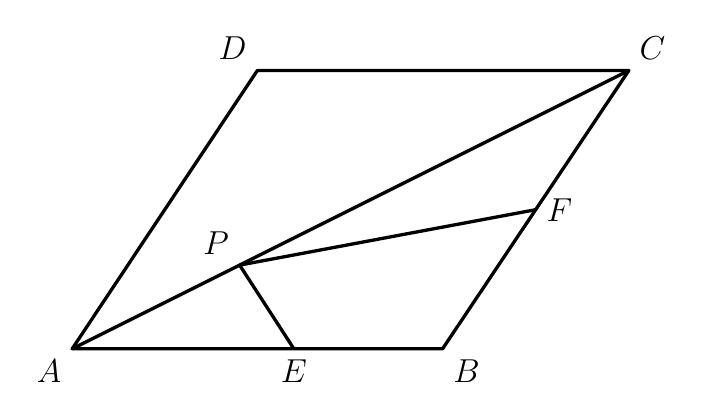
\begin{tikzpicture}[line width=1.2pt, line join=round, font=\fontsize{12}{14.4}\selectfont]
  % Vertices (converted from pixels)
  \coordinate (A) at (-3.550,-1.760);
  \coordinate (B) at (1.154,-1.760);
  \coordinate (C) at (3.520,1.775);
  \coordinate (D) at (-1.198,1.775);
  % Points on segments
  \coordinate (E) at (-0.734,-1.760);
  \coordinate (P) at (-1.423,-0.697);
  \coordinate (F) at (2.337,0.007);

  % Parallelogram sides and diagonal
  \draw (A) -- (B) -- (C) -- (D) -- cycle;
  \draw (A) -- (C);
  % Auxiliary segments
  \draw (P) -- (E);
  \draw (P) -- (F);

  % Labels
  \node[below left] at (A) {$A$};
  \node[below right] at (B) {$B$};
  \node[above right] at (C) {$C$};
  \node[above left] at (D) {$D$};
  \node[below] at (E) {$E$};
  \node[right] at (F) {$F$};
  \node[above left] at (P) {$P$};
\end{tikzpicture}
\end{document}